\label{chapter:sherifftools}

False sharing is a well-known performance issue~\cite{falseshare:effect, falseshare:Analysis}. We have discussed this problem in Section~\ref{sec:falsesharingproblems}. 

Detecting false sharing requires tools support. Existing tools share a similar shortcoming, where they can not pinpoint the exact place with false sharing problems, leaving the burden of finding actual places to programmers. Besides that, existing tools suffer from one or more different shortcomings.  Simulation based approaches ~\cite{falseshare:simulator} and binary instrumentation based approaches~\cite{falseshare:binaryinstrumentation1, falseshare:binaryinstrumentation2} normally introduce very significant performance overhead, slowing down the execution over $100\times$. Hardware performance counter based approaches generally provide much better performance, but they cannot differentiate false sharing from true sharing problems~\cite{detect:ptu, detect:intel}.

We provide two systems, \SheriffDetect{} and \SheriffProtect{}, to tackle with false sharing problems, based on the \sheriff{} framework that discussed in Section~\ref{sec:sheriffframework}. \Sheriff{} is a drop-in replacement of the standard \pthreads{} library, but providing ``per-thread'' protection and isolation mechanism. \SheriffDetect{} detects false sharing problem accurately (without false positives) and precisely, by pointing out the exact places with false sharing problems. It is also very efficient, only introducing 20\% performance overhead.  \SheriffProtect{} automatically tolerate false sharing problems when rewriting an application to resolve false sharing is infeasible or impractical. The reasons can be caused by either source code is unavailable, or padding data structures would degrade performance because of reduced cache utilization and/or increase memory footprint.


%\section{\sheriff{} Framework}
%\input{sheriff/overview}

\section{Detecting False Sharing}
\label{sec:detectfalseshare}

This section first describes the basic idea of detecting false sharing. 

\subsection{Basic Idea}
\label{sec:detectionidea}
False sharing occurs when more than two threads concurrently access independent data within the same cache line, at least one of them are writes. False sharing does not necessarily cause performance problems. It can greatly degrade performance only when those accesses, caused by threads running on different cores with separate cache, actually cause a big number of cache invalidations. This is our \textbf{basic observation}. 

Generally, there are two known approaches to know how many cache invalidations actually occurring on a specific cache line, but they all suffer different shortcomings. 

The first approach relies on the underlying hardware, called as ``hardware-based approach''. We may rely on specific hardware performance counters, existing in some special hardware but not all, to know this information. But we cannot have thorough information about cache invalidations since existing mechanisms are based on sampling, which can lost a lot of information. Also, a tool based on this approach cannot apply to a different hardware that do not have specific hardware support. 

The second approach is to simulate the cache activity on different cache lines. To do that, we have to know all hardware-related information, including cache hierarchy, cache capacity and cache eviction rule, and the relationship between a thread and a specific core (that is hard to match actual situation). Even worse, simulation-based approaches are normally very slow and cannot be generalized to an execution running on a different hardware environment. 

To avoid these problems, we provide a software-only and generalized approach that can only rely on memory access history of each cache line, which is used by both \SheriffDetect{} and \Predator{} (discussed in Section~\ref{chapter:preditor}). Our approach is based on two conservative assumptions.
  
{\it First assumption:} 
All threads are running on different cores, with separate caches. Using this assumption can avoid knowing actual hardware cache hierarchy and the running situation between a thread and different cores. Although in a particular execution, two threads may run on the same core, thus reducing the effect of possible false sharing problems. Assuming that two threads are running on different cores can always represent a worst-case scenario that can happen in future executions. Thus, this assumption is very conservative, helping report any possible false sharing problem. 

{\it Second assumption:} 
A cache entry is never evicted from its private cache by cache eviction, meaning that all caches have infinite capacity. This assumption allows us to compute a cache invalidation without considering whether this entry is still in the cache or not. 

These two assumptions together allow us to compute cache invalidations based on memory accesses only. Based on these assumptions, we have the following {\bf observation}: there is a cache invalidation if a thread writes a cache line after another thread's access on the same cache line. Because the last thread accessing this cache line creates a copy of the same cache line on its running core's private cache (first assumption) and holds this copy(second assumption), this write operation definitely causes a cache invalidation, which invalidates the data copy on the core accessed by last thread. 


\begin{figure}[!t]
\centering
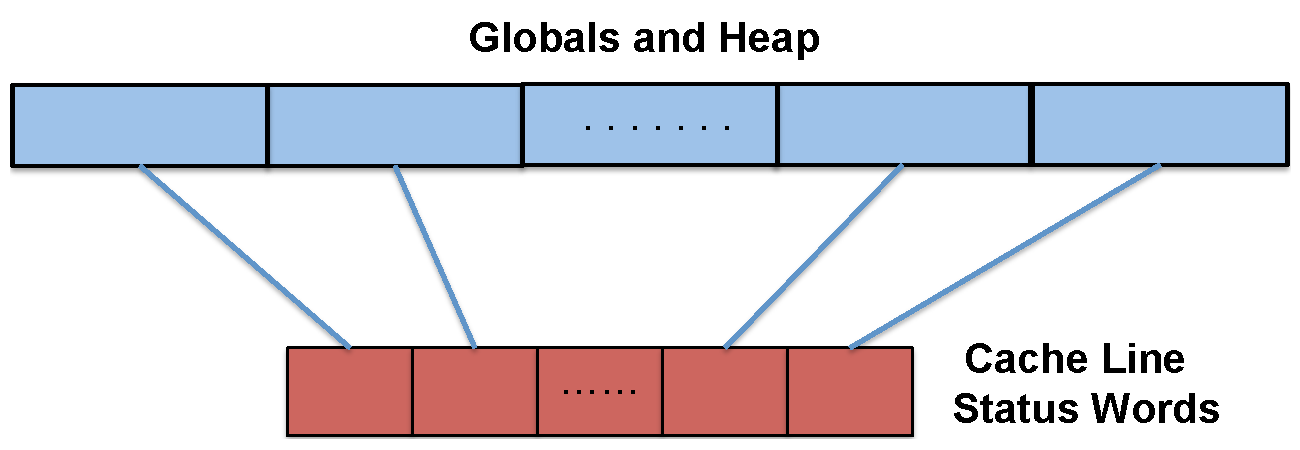
\includegraphics[width=6in]{fig/cachelinestatuswords}
\caption{
To detect false sharing, each cache line of the globals and heap maintains a cache line status word, which is updated on each memory access. \label{fig:cachelinestatusword}}
\end{figure}


To locate cache lines with a big number of cache invalidations, we maintain a cache line status word for each cache line in the globals and heap, shown in Figure~\ref{fig:cachelinestatusword}. We share a similar mechanism as another concurrent work of Zhao et.al. ~\cite{qinzhao}. 
However, the detailed implementation is totally different. Zhao et.al. utilize the detailed ownership bitmap to track those cores that have a duplicate copy of data, which can even track how many cache invalidations may happen in a write operation. However, their design cannot be easily scaled to more than 32 threads, requiring more memory overhead caused by more bits and more checking performance overhead. Also, their approach misses one important factor -- how many cache invalidations happening on a specific cache line. Without this information, it is impossible to pinpoint false sharing problems that can cause performance problems.
Our approach overcomes these shortcomings, by only tracking the last thread index and the number of cache invalidations.  Thus, we can rank the seriousness of false sharing problems based on the number of cache invalidations.
 

\subsubsection{Accurate Detection}
\label{sec:accuratedetect}
Accurate detection implies that we only report those false sharing problems that can cause performance problems. We employs the following mechanisms to avoid false positives.

First, we only report false sharing problems with a big number of cache invalidations, larger than a pre-defined but changeable threshold, thus can potentially cause performance problems. Utilizing the number of cache validations as an indicator avoids the problem of some existing tools, like PTU~\cite{detect:ptu, detect:intel}. PTU aggregates memory accesses without considering memory access interleaving, which  can report some cases that has a big number of memory accesses but without many cache invalidations. 

Second, we can differentiate false sharing from true sharing since true sharing can also cause cache invalidations. To do this, Zhao et.al. update bitmaps for every read and write in order to precisely determine whether an invalidation is related to a false sharing or a true sharing ~\cite{qinzhao}. However, this approach brings scalability problem that can not scale to more threads, bringing more memory overhead. We achieve the same target differently: we do not differentiate false sharing from true sharing during normal executions, but only track word-level accesses information: how many reads or writes are issued by which thread, where a word accessed by multiple threads is as ``shared''. This design lets us accurately distinguish false sharing from true sharing in the reporting phase, while do not have the scalability issue. It also helps diagnose where actual false sharing occurs when there are multiple fields or multiple objects in the same cache line, as this can greatly reduce the manual effort required to fix the false sharing problems.

  
Third, we can avoid pseudo false sharing (false positives) caused by memory reuses.  We intercept those memory allocations and deallocations, update information at memory deallocations for those objects without false sharing problems; heap objects involved in false sharing are never reused so that they can be reported in the end or on demand.


\subsubsection{Precise Detection}
\label{sec:precisedetect}

Precise detection implies that we can precisely point out where the problem is. Thus, programmers can leverage on that to identify and correct false sharing problems.

For global variables, we identify the name of global variables involving in false sharing problems, by looking up corresponding debug information. For heap objects, we report the callsite of those memory allocations by presenting the line of source code. In order to capture the origins of heap objects, we intercept those intercepting memory allocations and deallocations and use different ways to get callsite information, which are discussed in Section~\ref{sec:sheriffcallsite} and Section~\ref{sec:predatorcallsite}.

To help programmers precisely identify culprits of performance problem, we also present word-level accesses information so that the exact variables or fields that cause performance problems can be determined precisely. 

\subsubsection{Flexible Reporting}
\label{sec:flexiblereport}

We provide two different ways to report those false sharing problems. Normally, we can report those false sharing problems in the end of a program. However, this way does not work for those long-running applications. Thus, we provide a on-demand reporting way. User can send a specified signal to those applications that are installed with our tool. By intercepting those signals, we can report false sharing problems on demand.

In order to find out those cache lines with false sharing problems, we scan cache line status words of all memory, including the globals and heap, and only report those false sharing problems that can possibly cause performance problems, with the number of cache invalidations larger than a pre-defined but adjustable threshold.

\subsection{Detailed Implementations}

\label{sec:sheriffdetect}
\SheriffDetect{} relies on the \sheriff{} framework to track memory writes, thus detecting the write-write type of false sharing problems.  

%%% Tongping Liu
\subsubsection{Tracking Memory Accesses}
\label{sec:memoryaccesses}

\begin{figure*}[!t]
\centering
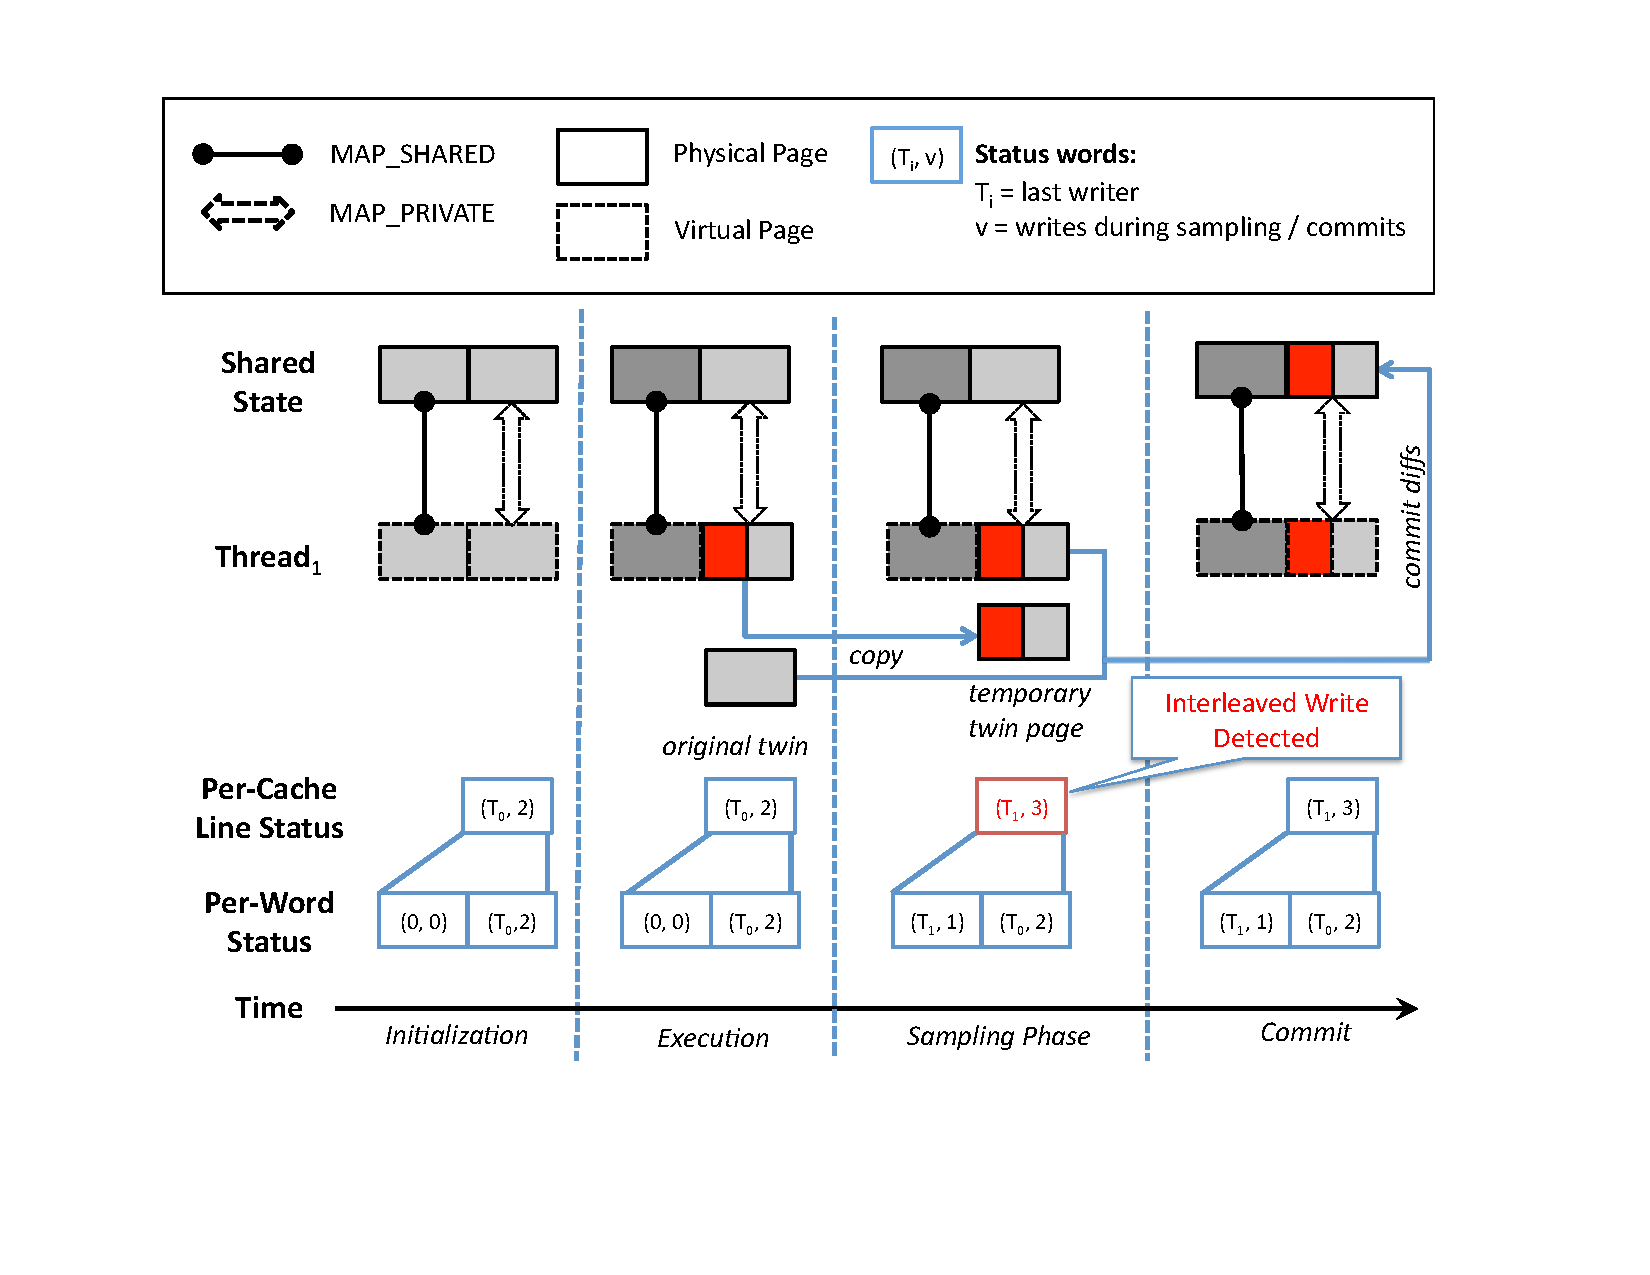
\includegraphics[width=6in]{sheriff/figure/sheriffdetective.pdf}
\caption{
Overview of \SheriffDetect{}’s operations. \SheriffDetect{} extends \Sheriff{} with sampling, per-cacheline status arrays, and per-word status arrays. For clarity of exposition, the diagram depicts just one cache line per page and two words per cache line.\label{fig:sheriffdetect}}
\end{figure*}

As discussed in Section~\ref{sec:detectionidea}, we can detect cache invalidations only based on memory accesses: for every memory access, we check recent memory access history, update the number of cache invalidations if possible, and update corresponding memory access history. 
Base on our observation, if the current access is a write, and other threads have accessed this cache line since last invalidation, then there is a cache invalidation. 
The \sheriff{} framework isolates executions from different threads, only commits those changes of different threads to the shared mapping at synchronization boundaries. Thus, by comparing a ``working'' page against its ``twin'' page,  \sheriffDetect{} can discover those accumulative memory writes  that occurred in the last transaction.  

However, if a transaction is long-running, finding memory changes at the end of every transaction is not enough 
to find those false sharing problems happening in the middle of a transaction. For example, the \texttt{linear\_regression} benchmark (described in Section~\ref{sec:evaluation}), 
degrading the performance by more than $10\times$ because of its false sharing problem, only has a single transaction per thread. 

In order to detect memory writes in the middle of an transaction, \SheriffDetect{} employs a sampling mechanism, employing the timer mechanism of the underlying operating system. 
We utilize the \texttt{alarm} library API to generate a periodical alarm to our detection system: by handling the \texttt{SIGALRM} signal, \SheriffDetect{} tracks memory writes accumulatively in the current period using the twinning-and-diffing mechanism (section~\ref{sec:twinning-and-diffing}). To do this, \SheriffDetect{} also keeps and updates a ``temporary twin'' page at every alarm interval, by simply copying from its ``working'' page. The difference between a ``working'' page and its ``temporary'' page implies those memory writes happening in the current sampling period. 

Currently, \SheriffDetect{} samples memory accesses of each thread at every 10 microsecond, which is  adjustable in our implementation. More frequent sampling may uncover more false sharing problems, but at the cost of increasing performance overhead. The tradeoff between effectiveness and performance overhead is further discussed and evaluated in Section~\ref{sec:results-sampling-overhead}. 

\subsubsection{Tracking Cache Invalidations}
\label{sec:invalidation}
As the discussion in Section~\ref{sec:detectionidea}, \SheriffDetect{} tracks and reports those cache lines with a big number of cache invalidations, which may cause serious performance problems. 

In order to track cache invalidations, \SheriffDetect{} introduces a cache line status word for every cache line of the globals and heap, showed in Figure~\ref{fig:cachelinestatusword}.  \SheriffDetect{} introduces two fields for every cache line status word, the last thread writing to this cache line and the number of cache invalidations of this cache line. 
Every time, when \SheriffDetect{} tracks a memory write, either at the end of each transaction or during the sampling timer handler, it updates these two fields correspondingly. Based on the assumptions described in Section~\ref{sec:detectionidea}, \SheriffDetect{} increments the number of cache invalidations when there is a write from a different thread and changes the last thread to the current thread (by recording thread id). To avoid using lock, \SheriffDetect{} updates those counters using atomic primitives. Since we base on thread id to identify whether there is a cache invalidation, without keeping track of detailed ownership id, this approach can scale up to any number of threads.   

\subsection{Optimizations}

\SheriffDetect{} employs the following optimizations in order to reduce its performance overhead. 

\paragraph{Getting Callsite Information.}
\label{sec:sheriffcallsite}

\SheriffDetect{} intercepts memory allocation operations in order to collect callsites for every heap object. To reduce the performance overhead, \SheriffDetect{} does not use the \texttt{bracktrace()} function call, but identify the callsite by analyzing the return or frame address using GCC extensions. However, this can not work on applications without debugging information. 

\paragraph{Reducing timer overhead.}
As explained in Section~\ref{sec:memoryaccesses}, \SheriffDetect{} uses a sampling mechanism to track cache invalidations. To reduce the performance overhead caused by by handling those alarm signals, \SheriffDetect{} activates sampling only when the average transaction time is larger than a pre-defined threshold (currently 10 milliseconds). \SheriffDetect{} uses an exponential moving average to track the average transaction time ($\alpha = 0.9$). This optimization does not significantly reduce the possibility of finding false sharing, since \SheriffDetect{} can track those accumulative writes inside every short transaction by checking only at the end of transactions.

\paragraph{Sampling to find shared pages.} 
If an application has a large number of transactions or a large memory footprint, the overhead of handling page protection can dominate the total running time.
To reduce the number of pages that should be tracked, \SheriffDetect{} leverages a
simple insight: if two threads can falsely share (write-write share) a cache line, then they must simultaneously write to the same page containing this cache line. 
Leveraging on this insight, \SheriffDetect{} only tracks those pages written by multiple threads. 

In order to identify those shared pages, \SheriffDetect{} is based on the following assumption: if objects on a page are frequently falsely shared, the corresponding page must also be frequently shared; thus, even relatively infrequent sampling on memory accesses can reveal the shared relationship. \SheriffDetect{} currently samples the first 50 out of every 1,000 periods (one period equals one transaction or one sampling interval). At the beginning of each sampling period, all memory pages are made read-only so that any
writes to each page will be detected. Upon finding a page that is shared across multiple threads, \SheriffDetect{} tracks all memory accesses happening on this page, thus possibly finding any false sharing inside this page. 

By using this sampling mechanism, those pages, with sharing status unknown, impose no protection overhead at all. \sheriffDetect{} only pays protection overhead for those shared pages outside the sampling period, instead of all memory pages. 

\subsection{Limitation}
\label{discussion:faultofdetect}

Unlike previous tools, \SheriffDetect{} reports no false positives, differentiates true sharing from false sharing, and avoids false positives caused by the reuse of heap objects. 

However, \SheriffDetect{} can under-report false sharing instances in the following situations:

\paragraph{Single writer.}
False sharing usually involves concurrent updates from multiple threads. But it can also arise when there is exactly one thread writing to part of a cache line while other threads read from this cache line. 
Because \sheriffdetect{} can only track writes, it cannot detect this single-writer false sharing, missing some false sharing problems. 

\paragraph{Heap-induced false sharing.}  
\sheriff{} replaces the standard memory allocator with one that, like the Hoard allocator, avoids most heap-induced false sharing. \sheriff{}'s memory allocator (like Hoard), carves memory into page-sized chunks; each thread allocates from its own set of chunks, and the allocator never splits cache lines across threads. Because \SheriffDetect{} uses a different custom memory allocator, it cannot detect false sharing that is caused by using the standard memory allocator. Since it is straightforward to deploy Hoard or a similar allocator to avoid heap-induced false sharing, this limitation is not a problem in practice.

\paragraph{Misses due to sampling.}  Since it uses sampling to find shared pages, \SheriffDetect{} may fail to track those pages that written in the middle of sampling intervals. We hypothesize that false sharing instances that affect performance are unlikely to perform frequent writes exclusively during that time, and so are unlikely to be missed.


\section{Tolerating False Sharing}
\label{sec:sheriffprotect}
While \SheriffDetect{} can effectively find those false sharing problems of multithreaded programs, it is sometimes difficult or impossible to fix them. For example, padding memory to avoid false sharing may even slowdown the performance because of excessive memory consumption or reducing cache utilization~\cite{qinzhao}. Also, time constraints or unavailable source code may prevent the fixes. 

Based on the \sheriff{} framework, we provide the second tool, \SheriffProtect{}, to automatically boost the performance for multithreaded applications with false sharing problems, without programmer intervention.  

\SheriffProtect{} borrows the insight initially introduced by Dubois et.al.~\cite{Dubois:1991:DCE:125826.125941}: {\it delaying updates avoids false sharing}. Because \Sheriff{} replaces threads with processes, executions of different threads are actually isolated from each other. Thus, different ``threads'' (processes) actually access different physical pages (and cache lines), when originally they are accessing the same cache line in the multithreading environment. This helps avoid false sharing problems. 

However, simply using the \sheriff{} framework introduces excessive performance overhead because of the following reasons: 

\begin{itemize}
\item
The overhead of protecting and committing all pages may be too high. As we already know in Section~\ref{sec:sheriffframework}, \sheriff{} has to commit all local changes of different threads  to the shared mapping at the end of every transaction (synchronization points) in order to achieve the shared memory semantics. 

\item
If the length of a transaction is short, the overhead of protecting and committing pages in the \sheriff{} framework can be easily higher than the performance benefit by tolerating possible false sharing problems inside. Thus, there is no benefit to tolerate false sharing problems for short-running transactions. 

\end{itemize}

\sheriffprotect{} provides two corresponding mechanisms to avoid these possible overhead. 

\emph{Selective Protection.} 
\SheriffProtect{} only prevents false sharing on small objects, with size less than 1024 bytes. All large objects are mapped shared and are never protected, thus can not tolerate false sharing problems caused by these large objects. We expect  small objects to be a likely source of false sharing because more of them can fit on a cache line. Also, for large objects, the cost of protecting and committing changes can be bigger than the benefit of tolerating possible false sharing problems inside. 

\emph{Adaptive Prevention.}
\SheriffProtect{} employs a simple adaptive mechanism: it only isolates threads' executions if the average transaction length is large than a pre-set threshold. \SheriffProtect{} keeps track of the length of each transaction and uses a exponential weighted averaging ($\alpha = 0.9$) to calculate the average transaction length. If the average transaction length falls below an established threshold, \SheriffProtect{} switches to the shared mappings for all memory and does no further page protections. As long as transactions remain too short, 
 without any benefit to tolerate false sharing problems inside, the protection mechanisms remain switched off. If the average transaction length rises back above the threshold, \SheriffProtect{} re-establishes private mappings and page protections, thus avoiding possible false sharing to achieve better performance.

\section{Experimental Evaluation}
\label{sec:evaluation}

We perform all of our evaluations on a quiescent dual processor (totally 8 cores) system with 8GB of RAM. Each processor is a 4-core 64-bit Intel Xeon, running at 2.33 GHz with a 4MB L2 cache. For compatibility reasons, we compile all applications to a 32-bit target using the GCC compiler. All performance data is the average of ten runs, excluding the maximum and minimum values.

The evaluation answers the following questions:

\begin{itemize}
\item How effective is \sheriffdetect{} at finding false sharing and guiding programmers to their resolution? (Section~\ref{sec:effecteval})
\item What is \sheriffdetect{}'s performance overhead? (Section~\ref{sec:results-runtime-overhead})
\item How sensitive is \sheriffdetect{} to different sampling rates? (Section~\ref{sec:results-sampling-overhead}) 
\item How effective does \sheriffprotect{} mitigate false sharing? (Section~\ref{sec:protectperformance})
\end{itemize}

\subsection{Detection Effectiveness}

\label{sec:effecteval}

This section evaluates whether \sheriffdetect{} can be used to find false sharing problems, both in synthetic test cases and in actual applications.

We developed a range of microbenchmarks that exemplify different situations related to false sharing. We evaluate these benchmarks on both \SheriffDetect{} and Intel's Performance Tuning Utility(PTU v3.2), the previous state-of-the-art work of false sharing detection. 

Detection results are shown in Table~\ref{table:microbenchmarks}. \sheriffdetect{} only reports those false sharing instances that can possibly affect performance, while correctly ignores those cases without performance impact.
PTU has false alarms/positives.  It does not track access patterns, which reports false positives for those non-interleaved accesses. Also, PTU does not track memory deallocations, thus it can not filter out those pseudo false sharing caused by memory reuse. \sheriffdetect{} avoids all of these problems and reports false sharing problems correctly. 


\begin{table}
\centering
\resizebox{\columnwidth}{!}{
\begin{tabular}{l|l|l|l}
\hline
{\bf \small Microbenchmark} & {\bf \small Perf Sensitive } & {\bf \small \sheriffdetect{} } & {\bf \small PTU } \\
\hline

\small \textbf{False Sharing (adjacent objects)} & YES & \cmark{} & \cmark{} \\
\small \textbf{False Sharing (same object)} & YES & \cmark{} & \cmark{} \\
\hline
\small \textbf{True Sharing} & NO & & \\
\small \textbf{Non-interleaved False Sharing} & NO & & \xmark{}\\
\small \textbf{Heap Reuse(no sharing)} & NO & & \xmark{}\\
\hline
\end{tabular}
}
\caption{False sharing detection results using PTU and \sheriffdetect{}. \sheriffdetect{} correctly reports only actual false sharing instances that have performance impact;
\cmark{} indicates a correct report and \xmark{} indicates a false alarm. 
\label{table:microbenchmarks}}
\end{table}

We further evaluate \SheriffDetect{} and PTU on two widely-used benchmark suites, Phoenix~\cite{phoenix-hpca} and PARSEC~\cite{parsec}. We use the simlarge inputs for all applications of PARSEC. For Phoenix, we choose available parameters that allow the programs to run as long as possible. We were unable to successfully compile \texttt{raytrace} and \texttt{vips}, and \sheriff{} is currently unable to run \texttt{x264}, \texttt{bodytrack}, and \texttt{facesim}. \texttt{Freqmine} currently can not support \pthreads{}. Thus, those benchmarks are excluded here. 
 
\begin{table}
\centering
\begin{tabular}{l|r|r}
\hline
{\bf \small Benchmark} & {\bf \small PTU} & {\bf \small \sheriffdetect{}}\\
 & {\# Lines} & {\# Objects}\\
\hline
\small \textbf{kmeans} & 1916 &  2 \\
\small \textbf{linear\_regression} & 5 & 1 \\
\small \textbf{matrix\_multiply} & 468 & 0\\
\small \textbf{pca} & 45 & 0 \\
\small \textbf{reverseindex} & N/A & 5 \\
\small \textbf{word\_count} & 4 & 3\\
\hline
\small \textbf{canneal} & 1 & 1 \\
\small \textbf{fluidanimate} & 3 & 1 \\
\small \textbf{streamcluster} & 9 & 1\\
\small \textbf{swaptions} & 196 & 0\\
\hline
\small \textbf{Total} & 2647 & 14\\
\hline
\end{tabular}
\caption{Overall detection results of PTU and \sheriffdetect{} on Phoenix and PARSEC benchmark suites. We only list those benchmarks that at least one of tools reports false sharing problems. For PTU, we show how many cache lines are marked as falsely shared. For \sheriffdetect{}, we show how many objects are reported by \sheriffdetect{} (with cache invalidations larger than 100). The item marked as ``N/A'' means that PTU fails to show results because it runs out of memory.
\label{table:fsdetection}}
\end{table}


The overall results are shown in Table~\ref{table:fsdetection}. PTU reports that 2647 cache lines may exist false sharing problems. \sheriffdetect{} reveals that seven out of sixteen evaluated benchmarks have false sharing problems. Totally, only 14 objects are reported, but only 4 of them shows a big number of cache invalidations, thus needs to be fixed. 

Several reasons contribute to the number difference between these two approaches. First, PTU reports cache lines involving in false sharing, while \SheriffDetect{} only reports objects. If an object has a size larger than the size of cache line, PTU can report multiple times, one on each cache line. Second, PTU reports multiple times if a heap object, with the same allocation site, is allocated multiple times, while \SheriffDetect{} only reports once. Third, PTU may report false positives since it does not track interleaved accesses and overrates the problems caused by heap reuses. 

We manually fix these four false sharing problems based on reports of \SheriffDetect{}, and show the performance gains after fixes in Table~\ref{table:perfafterfix}. To explain why performance improvement are different, we also examine the maximum possible updates that can occur on a false sharing object, although the actual number of interleaved accesses depends on actual scheduling. For example, \texttt{linear\_regression} has the largest updates, thus causing the most serious performance problem. 

\begin{table}
\centering
\begin{tabular}{l|r|r}
\hline
{\bf \small Benchmark} & {\bf \small Performance Improvement} & {\bf \small Updates}\\
 & & (M)\\
\hline
\small \textbf{linear\_regression} & 818\% & 1323.6\\
\small \textbf{reverseindex} &  2.4\% & 0.4\\
\small \textbf{streamcluster} & 5.4\% & 28.7\\
\small \textbf{word\_count} &  1\% & 0.3\\
\hline
\end{tabular}
\caption{Performance data for four false sharing benchmarks. All data are obtained using the standard \pthreads{} library. ``Updates'' shows how many million updates (in total) occurred on falsely-shared cache lines.
\label{table:perfafterfix}}
\end{table}


In \texttt{reverse\_index} and \texttt{word\_count}, multiple threads repeatedly modify the same heap object. The pseudo code for these two benchmarks are listed in Figure~\ref{fig:reverseindex}. For these two benchmarks, we can use thread-local variables to avoid performance problems: each thread can operate on a temporary variable first, and then modify the \texttt{use\_len} array at the end.

\begin{figure}[!t]
\begin{lstlisting}[style=tt]
int * use_len;
void insert_sorted(int curr_thread) {
   ......	
   // After finding a new link
   (use_len[curr_thread])++;
   ......	
}
\end{lstlisting}
\caption{A fragment of source code from \texttt{reverse\_index}. False sharing arises when different threads 
modify different words in the same \texttt{use\_len} array. 
\label{fig:reverseindex}}
\end{figure}

\texttt{Linear\_regression}'s false sharing problem is a little different (see Figure~\ref{fig:linear_regression}). 
Two different threads write to two independent parts of the same cache line, when these parts (caused by the size of\texttt{lreg\_args} structure) are not large enough to occupy a cache line. This problem can be avoided easily by padding the structure \texttt{lreg\_args}, thus preventing different threads concurrently accessing the same cache line. 

\begin{figure}[!t]
\begin{lstlisting}[style=tt]
struct {
  long long SX;
  long long SY;
  long long SXX;
  ......
} lreg_args;

void *lreg_thread(void *args_in) {
  struct lreg_args * args = args_in;
  for(i = 0; i < args->num_elems; i++) {
    args->SX  += args->points[i].x;
    args->SXX += args->points[i].x 
   	         * args->points[i].x;
  }
  ......	
}
\end{lstlisting}
\caption{A fragment of \texttt{linear\_regression} code. Each thread works on its independent elements of the array. 
Unfortunately, the size of \texttt{struct lreg\_args} is not large enough (only 52 bytes) on 32-bit machine, which causing two different threads to write to the same cache line simultaneously. 
\label{fig:linear_regression}}
\end{figure}

The false sharing problem detected in \texttt{streamcluster} (one of the PARSEC benchmarks) is similar to that in \texttt{linear\_regression}: two different threads are writing to the same cache line. Examination of the source code indicates that the author tried to avoid false sharing by padding, but the amount of padding, 32 bytes, was insufficient to accommodate the actual physical cache line size used in the evaluation (64 bytes). Setting the \texttt{CACHE\_LINE} macro to 64 bytes reduces the effect of false sharing, improving the performance by 5.4\%.


\subsubsection{Ease of Locating False Sharing Problems}

\label{sec:fsfixexample}

To illustrate how \sheriffdetect{} can precisely locate false sharing problems, we use one benchmark (\texttt{word\_count}, a Phoenix benchmark) as an example. Diagnosing other false sharing issues is similar to this one.

Here is an example output from \sheriffdetect{} for \texttt{word\_count}.

\begin{verbatim} 
1st object, cache interleaving writes 
13767 times (start at 0xd5c8e140). 
Object start 0xd5c8e160, length 32. 
It is a heap object with callsite:
[0]: ./wordcount_pthreads.c:136
[1]: ./wordcount_pthreads.c:441
\end{verbatim}

Line 136 (\texttt{wordcount\_\pthreads{}.c}) contains the following memory allocation:

\begin{verbatim}
use_len=malloc(num_procs*sizeof(int));
\end{verbatim}

Grepping for \texttt{use\_len}, a global pointer, quickly leads to this line:

\begin{verbatim}
use_len[thread_num]++;
\end{verbatim}

Now it is very clear that different threads are modifying the same object(use\_len). Fixing the problem by using a thread-local data copy is now straightforward.

By contrast, we can compare PTU's output that shown in Figure~\ref{fig:wordcount}. Pinpointing the false sharing problem inside is far more complicated with PTU: it only reports functions involving in a questionable cache line, not to mention the fact that PTU can report huge numbers of false positives.  Another shortcoming of PTU is that ``Collected Data Refs'' number cannot be used as a metric to evaluate the significance of false sharing problems. For this example, PTU only reports 12 references, while \sheriffdetect{} observes 13767 cache invalidations.

\begin{figure*}[!t]
\centering
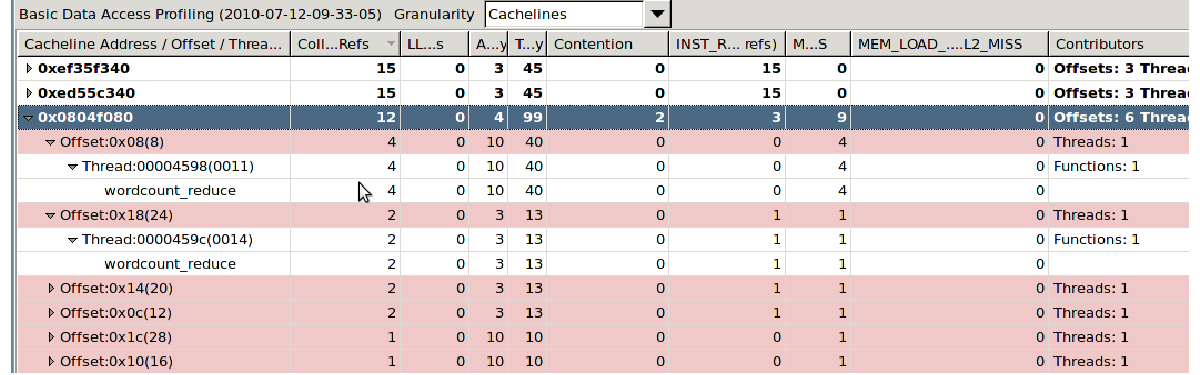
\includegraphics[width=6in]{sheriff/figure/wordcount}
\caption{PTU output for \texttt{word\_count}.
\label{fig:wordcount}}
\end{figure*}

\subsection{Detection Performance Overhead}
\label{sec:results-runtime-overhead}

\begin{figure*}[!t]
\centering
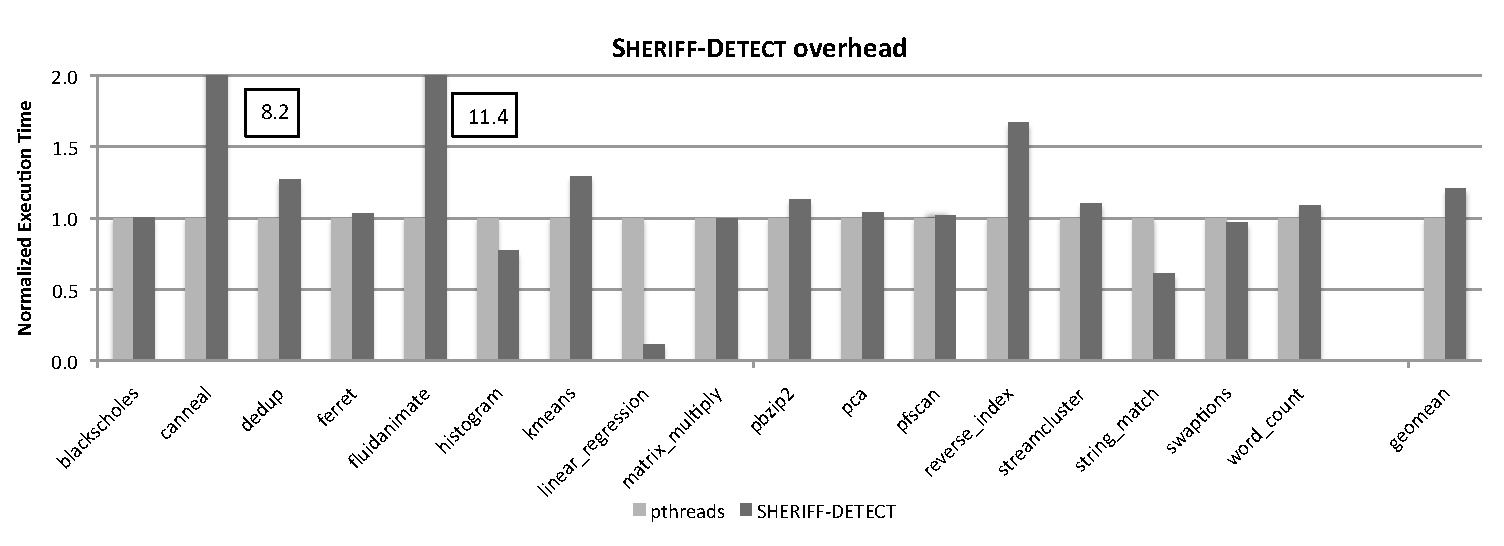
\includegraphics[width=6in]{sheriff/figure/detectiveperf.pdf}
\caption{\sheriffdetect{} performance overhead across two suites of benchmarks, normalized to the runtime of using the \pthreads{} library (lower is better). \label{fig:overhead}}
\end{figure*}


\SheriffDetect{}'s  runtime overhead (comparing to \pthreads{}) on two multithreaded benchmarks suites, Phoenix and PARSEC, is shown in Figure~\ref{fig:overhead}.  \SheriffDetect{} only introduces 20\% performance on average, with the exception of three outliers. For other benchmarks, \SheriffDetect{}’s overhead is generally acceptable and far lower than most existing tools.


\sheriffdetect{} do not perform well on two benchmarks. \texttt{canneal} runs about $7\times$ slower than that with \pthreads{}.  \texttt{fluidanimate}'s  performance overhead is about $11\times$ slower than that using \pthreads{}.

The first reason is that both benchmarks
trigger a high number of dirtied pages (3.4 million and
2.15 million, respectively). For each dirty page, \sheriffdetect{} applies page protection twice, creates a ``copy-on-write'' page and a ``twin'' page, checks false sharing problems at every sampling interval, and commits those local changes to the shared mapping. Thus, given large amount of dirty pages, copying overhead alone is very expensive and can dominate most of overhead. For example, \texttt{Canneal} invokes around 3.4 million dirty pages, thus leading to substantial overhead. 

Another reason for \texttt{fluidanimate} is that it invokes an unusually high number of transactions (16.7 million).  \SheriffDetect{} introduces page protection and commits overhead at every transaction boundary, thus, adding overhead if there are dirty pages.
 
 
However, even with these outliers that run slowly, the overhead of \SheriffDetect{} is generally acceptable
and far lower than most existing tools. \SheriffDetect{} actually improves performance by eliminating false sharing, using its process-as-threads framework. \SheriffProtect{} further reduces overhead as the next section describes.

\texttt{linear\_regression} runs $8\times$ faster with \SheriffDetect{} than with \pthreads{}, even with the added overhead of protection, memory commits, sampling and 
other mechanisms.  There is a serious false sharing problem inside (see Table~\ref{table:perfafterfix},) which both \sheriffdetect{} and \sheriffprotect{} eliminate automatically. Other cases where \sheriffdetect{}
outperforms \pthreads{} are also due to false sharing elimination. 


%%%%%%%%%%%%%%%%%%%%%%%%%%%%%%%%%%%%%%%5
%%%% Some data to list the effectiveness of this tool.
%%%%%% How many caches are carried for each test case. 
%%%%%% Whether all caches has false sharing problem.
%%%%%%%%%%%%%%%%%%%%%%%%%%%%%%%%%%%%%%%
\subsection{Detection Sampling Rate Sensitivity}
\label{sec:results-sampling-overhead}

\SheriffDetect{} employs the sampling mechanism to detect false sharing happening in long-running transactions. Sampling is only triggered when the length of a transaction exceeds a pre-defined threshold, usually 10ms. By handling those \texttt{SIGALARM} signals, \SheriffDetect{} tracks memory accesses by by comparing the temporary twin page against its
corresponding working version, and updates status words of specific cache lines. Thus, increased sampling rates may uncover more false sharing problems, but at the cost of increase performance overhead. 

To measure \sheriffdetect{}'s sensitivity to different sampling rates, we evaluate on three different sampling rates: 2ms, 10ms (our baseline), and 50ms.

\paragraph{Sampling Overhead:} Figure~\ref{fig:sensitivity} shows the performance overhead under different sampling rates, normalized to the runtime of using the default 10ms sample rate. For most of these benchmarks, sampling imposes relatively little overhead either because the average
number of shared pages is small, or because the
transaction length is often shorter than the sampling interval (thus no adding checking overhead).

One outlier is \texttt{canneal}, which is extremely sensitive to a different sampling rate.  When the sampling rate is 2ms, \texttt{canneal} runs about $2.3\times$ slower than that with  a 10ms sampling rate; \texttt{canneal} runs 35\% slower with a 50ms sampling rate than 2 10ms
sampling rate. The reason is that \texttt{canneal} dirties a large number of shared pages. More frequent sampling thus creates more temporary ``twin'' pages and increases checking overhead.


\begin{figure*}[!t]
\centering
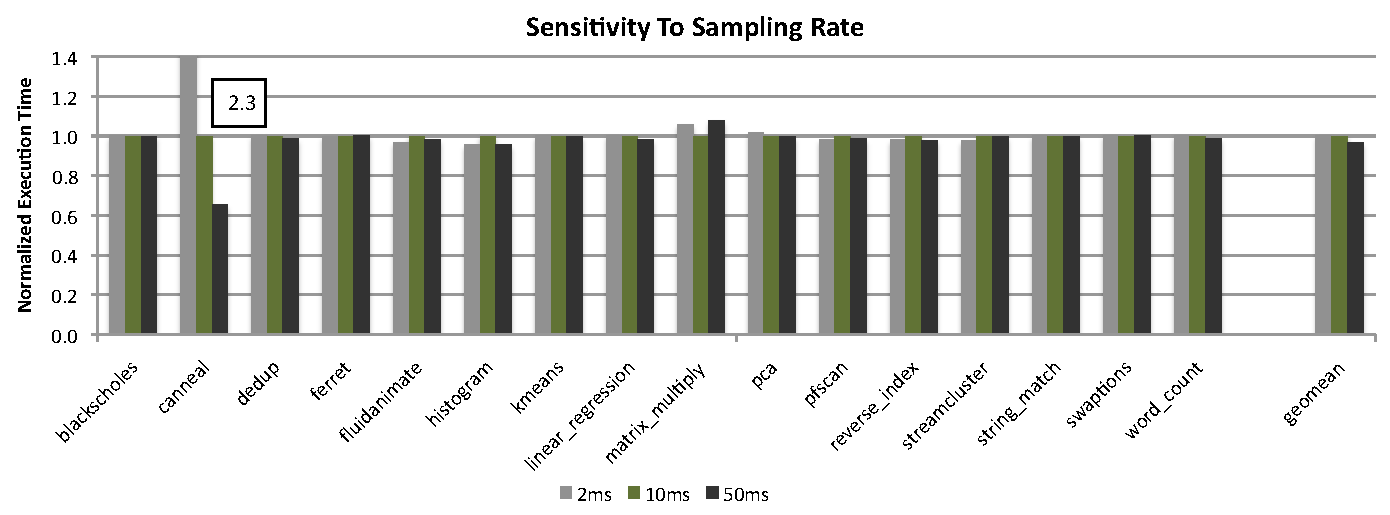
\includegraphics[width=6in]{sheriff/figure/sensitivity}
\caption{\sheriffdetect{} performance with different sampling rates,  normalized to the performance with a sampling interval of 10ms (presented in Figure~\ref{fig:overhead}); lower is better.
\label{fig:sensitivity}}
\end{figure*}

\begin{table*}[!t]
\centering
\resizebox{\columnwidth}{!}{
\begin{tabular}{l|rr|rr|rr}
\hline
{\bf \small Benchmark} & \multicolumn{2}{c|} {\bf \small 2ms} & \multicolumn{2}{c|} {\bf \small 10ms}& \multicolumn{2}{c} {\bf \small 50ms}\\
& {\em objs}  & {\em writes} & {\em objs}  & {\em writes} & {\em objs}  & {\em writes} \\
\hline
\small \texttt{canneal} & 1 & 21444321 & 1 & 26369324 & 1 & 30580451 \\
\small \texttt{ferret} & 1 & 3 & 0 & 0 & 0 & 0 \\
\small \texttt{fluidanimate} & 1 & 3370 & 1 & 4064 & 1 & 2851 \\
\small \texttt{kmeans} & 2 & 2974 & 2 & 1122 & 1 & 98 \\
\small \texttt{linear\_regression} & 1 & 1050 & 1 & 311 & 1 & 71 \\
\small \texttt{reverse\_index} & 5 & 14494 & 5 & 14782 & 5 & 14981 \\
\small \texttt{streamcluster} & 2 & 52462 & 1 & 52283 & 1 & 52420 \\
\small \texttt{word\_count} & 4 & 9849 & 4 & 2699 & 3 & 622 \\
\hline
\end{tabular}
}
\caption{
\sheriffdetect{} precision with different sampling rates, including the number of falsely-shared objects and interleaved writes. We omit those benchmarks with no observed cases of false sharing.
\label{table:samplingquality}}
\end{table*}

\paragraph{Sampling Effectiveness:}
The choice of sampling rates has relatively little impact on detection and ranking, shown in Table~\ref{table:samplingquality}. As expected, the number of falsely-shared objects reported and the number of interleaved writes observed are not significantly different.

Using a different sampling rate does affect the number of falsely-shared objects detected, but \SheriffDetect{} already reports all instances with a significant performance impact under the default sampling rate. Increasing the sampling rate to 2ms (more frequent sampling) reveals two additional falsely-shared objects (in \texttt{ferret} and \texttt{streamcluster}), but these two objects do not have a significant performance impact since they can only cause few cache invalidations(under 10). Similarly, reducing the sampling rate to 50ms (less frequent sampling) cannot detect two false sharing problems (in \texttt{kmeans} and \texttt{word\_count}), but these objects also have little impact on performance.


\subsection{Prevention Effectiveness}
\label{sec:protectperformance}

\begin{figure*}[!t]
\centering
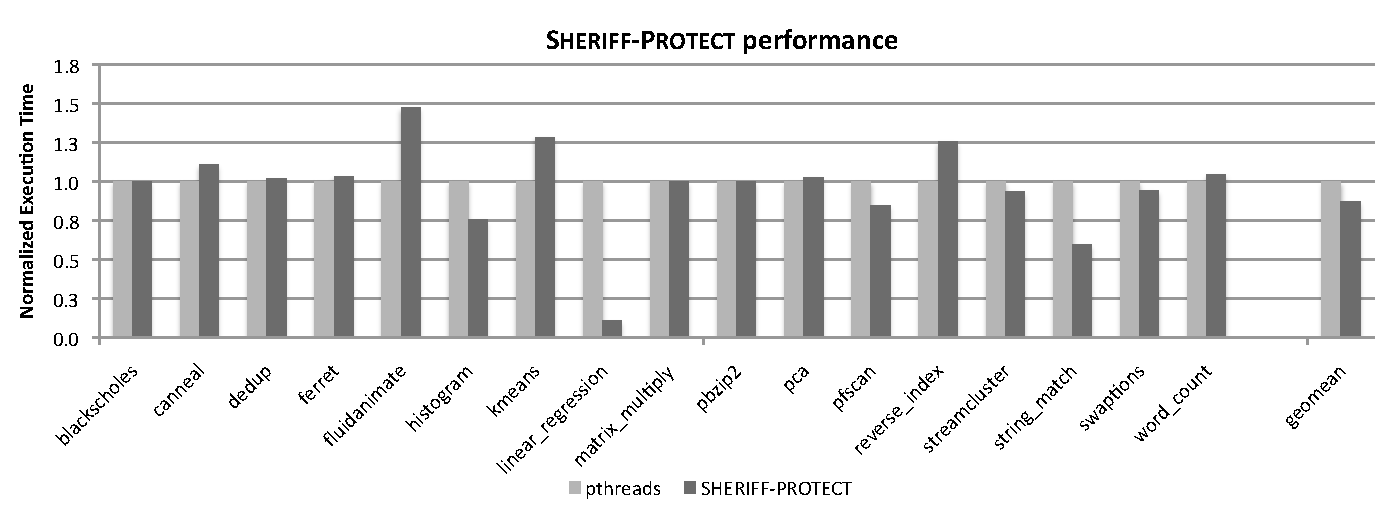
\includegraphics[width=6in]{sheriff/figure/patrolperf.pdf}
\caption{\sheriffprotect{} performance across two suites of benchmarks, normalized to the performance of \pthreads{} (see Section~\ref{sec:results-runtime-overhead}). In case of catastrophic false sharing, \sheriffdetect{} dramatically increases performance.
\label{fig:patrol}}
\end{figure*}

\begin{table}[!t]
\centering
\begin{tabular}{l|r|r}
\hline
{\bf \small Benchmark} & \multicolumn{2}{c} {\bf \small Normalized Runtime} \\
% \cline{2-3}
 & {\bf \small \sheriffdetect{} }  & {\bf \small \sheriffprotect{}} \\
\hline
\small \texttt{blackscholes} & 1.00 & 1.00 \\
\small \texttt{canneal} &  8.23 & 1.11 \\
\small \texttt{dedup} & 1.27 & 1.02 \\
\small \texttt{ferret} & 1.03 & 1.03\\
\small \texttt{fluidanimate} & 11.39 & 1.47 \\
\small \texttt{histogram} & \textbf{0.77} & \textbf{0.76} \\\small \texttt{kmeans} & 1.29 & 1.28 \\
\small \texttt{linear\_regression} & \textbf{0.12} & \textbf{0.11} \\
\small \texttt{matrix\_multiply} & 1.00 & 1.00 \\
\small \texttt{pbzip2} & 1.13 & 1.00 \\
\small \texttt{pca} & 1.04 & 1.03 \\
\small \texttt{pfscan} & 1.02 & \textbf{0.85} \\
\small \texttt{reverse\_index} & 1.67 & 1.25 \\
\small \texttt{streamcluster} & 1.10 &  \textbf{0.94} \\
\small \texttt{string\_match} & \textbf{0.61} & \textbf{0.60} \\
\small \texttt{swaptions} & \textbf{0.97} & \textbf{0.94} \\
\small \texttt{word\_count} & 1.09 & 1.05\\
\hline
\small \textbf{\em Geomean} & 1.21 & \textbf{0.87} \\
\hline
\end{tabular}
\caption{Detailed execution times with \sheriffdetect{} and \sheriffprotect{}, normalized to execution with the \pthreads{} library; numbers below 1 (boldfaced) indicate a speedup over \pthreads{}.
\label{table:detailedperf}}
\end{table}

We also examine the effectiveness of eliminating false sharing problems of using \SheriffProtect{}.  Figure~\ref{fig:patrol} presents the performance under \SheriffProtect{} and \pthreads{}.  For most cases, \SheriffProtect{} either has no effect on performance (when there is no false sharing problem inside) or improves the performance. Table~\ref{table:detailedperf} presents detailed performance results of \SheriffDetect{} and \SheriffProtect{}. 

\SheriffProtect{} improves the performance when an application is detected to have false sharing problems inside.  \texttt{linear\_regression} exhibits almost a $10\times$ speedup against the one using \pthreads{}, by tolerating a serious false sharing problem inside (see Table~\ref{table:perfafterfix}). \texttt{histogram} runs substantially faster with \SheriffProtect{} (24\%) because of preventing a read-write false sharing problem, see Section~\ref{sec:predatoreffective}. \texttt{string\_match} runs 40\% faster because of its custom memory allocator, preventing two threads allocating different objects from the same cache line, which is why \SheriffDetect{} does not find. 

Using \SheriffProtect{}, three benchmarks runs up to 47\% slower than using \pthreads{} because of different reasons. 
\texttt{kmeans} creates more than 3000 threads in eight seconds. Since the overhead of creating one process is higher than that of creating one thread, this dominates most of its overhead. For \texttt{reverse\_index} and \texttt{fluidanimate}, they exhibit slowdown because of using the processes-as-threads framework: Operating on those file-based pages is more expensive than operating on anonymous pages (the normal status of heap pages) under the Linux operating system; Writing to one page (\texttt{MAP\_SHARED}) cause a Copy-On-Write operation in the kernel even when there is only one user.  

Because \texttt{fluidanimate} has an enormous number of transactions(18 Million), \sheriffprotect{} 
introduces some additional overhead for every transaction. That also accounts for part of overhead.

